%-----------------------------------------------------------------------------%
\chapter{\babEmpat}
%-----------------------------------------------------------------------------%
Dalam bab ini akan dijelaskan hasil kalkulasi yang didapat dari implementasi numerik yang telah dikerjakan sesuai diagram pada bab 3. Kami memulainya dahulu dengan menghasilkan kembali hasil-hasil yang telah disepakati secara umum yakni melalui penyelesaian metode medan rata-rata dan iterasi pertubasi teori sebagai metode penyelesaian impuritas pembanding. Kami membagi hasil menjadi dua kelompok, yakni hasil dengan keadaan sistem untuk daerah paramagnetik dan antiferromagnetik. Dari model Hubbard, kami set besar nilai energi kinetik atau \textit{hopping} $t = 0.5$ eV. Parameter fisis lainnya, seperti temperatur $T$ dan interaksi elektron-elektron secara lokal $U$ divariasikan. Hal ini dikarenakan $t$ dapat dilihat sebagai energi skala untuk sistem.

%-----------------------------------------------------------------------------%
\section{Keadaan Paramagnetik}
%-----------------------------------------------------------------------------%
Pada kasus paramagnetik, magnetisasi, yakni dalam hal ini jumlah okupansi kedua sub kisi dalam kisi bipartite bernilai nol, dan kedua okupansi bernilai sama. Hal ini memberikan kondisi dimana tidak adanya kontribusi dari diagram orde 1, atau hartree-fock. Sehingga metode penyelesaian impuritas medan rata-rata tidak mampu menampilkan keadaan paramagnetik, dikarenakan \textit{self-energy} dari medan rata-rata hanya kontribusi dari diagram hartree. Sehingga keadaan paramagnetik dilihat dari metode iterasi pertubasi teori dan okupansi fluktuasi.

Pertama, menggunakan iterasi pertubasi teori, dimana \textit{self-energy} sepenuhnya hasil kontribusi dari diagram orde-2, kami menghitung jumlah keadaan elektron (DOS) dan \textit{self-energy} terhadap variasi $U$ dengan temperatur $T = 0$, hal ini diperlihatkan oleh gambar 4.1. Kita lihat bahwa evolusi DOS menunjukkan terdapatnya puncak quasipartikel pada daerah energi fermi $\omega = 0$ dengan $U$ relatif rendah, hal ini menunjukkan adanya perilaku \textit{fermi liquid}. Pada $U$ yang sangat tinggi perilaku tersebut hilang, dan sepenuhnya menjadi sistem dengan elektron yang terlokalisasi, dimana terjadi transfer keadaan dari pita eksitasi quasipartikel ke pita Hubbard. Fitur puncak quasipartikel juga menjelaskan dengan baik mengapa terjadinya transisi logam-isolator. Kita perhatikan pula $U = 2.8$ adalah nilai interaksi yang sangat mendekati dengan interaksi kritis untuk terjadinya transisi logam ke isolator. Transisi ini bisa juga diperlihatkan dari perilaku \textit{self-energy}, dimana interaksi lokal $U$ mengakibatkan tingginya interaksi energi pada daerah energi fermi. Semakin bear $U$, maka semakin besar pula nilai daerah interaksi pada energi fermi. Pada isolator, lokalisasi diperlihatkan dengan besar dan kecilnya daerah energi pada \textit{self-energy}. Besarnya interaksi pada energi rendah membuat elektron terlokalisasi pada satu kisi, dan elektron cenderung menempati keadaan dengan energi relatif tinggi.
\begin{figure}
	\centering
	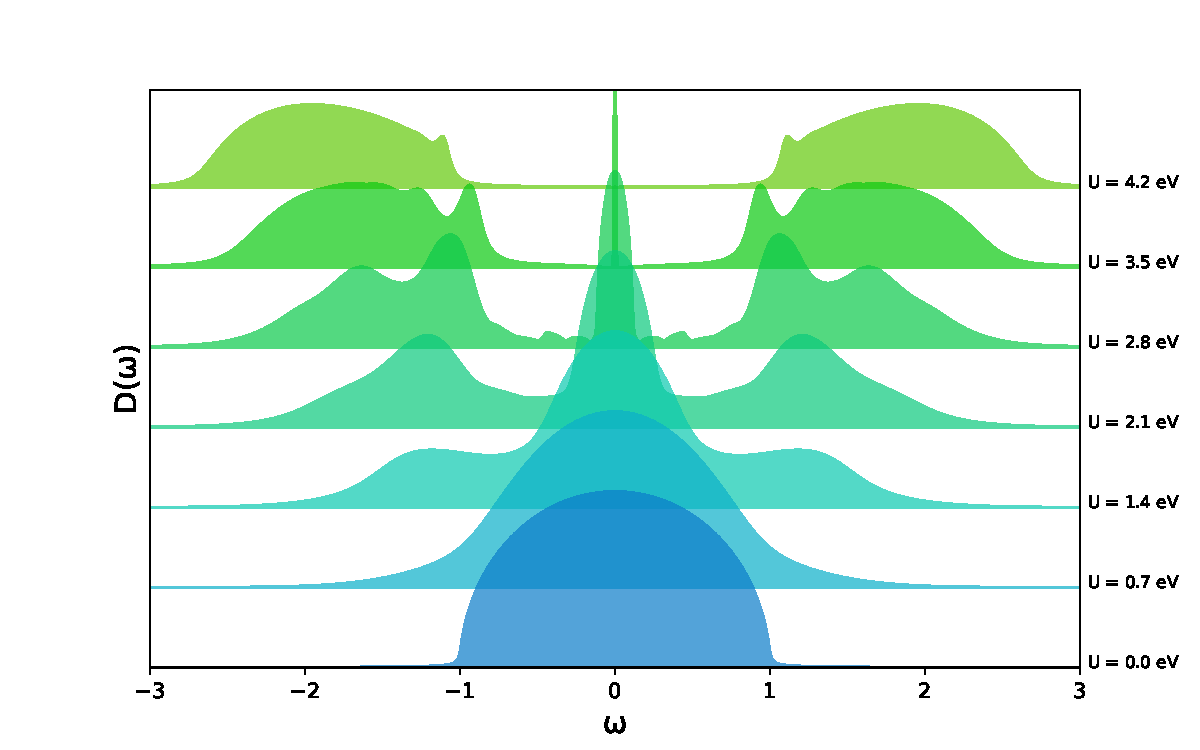
\includegraphics[width=1.00\textwidth]
		{pics/evolUDOS_IPT.pdf}
	\includegraphics[width=1.00\textwidth]
		{pics/evolUΣ2_IPT.pdf}
		\caption{(Atas) Evolusi DOS terhadap interaksi lokal $U$, dan (Bawah) Evolusi dari nilai imajiner \textit{self-energy} dari variasi $U$ yang sama pada temperatur $T = 0 K$ dengan menggunakan metode penyelesaian impuritas teori iterasi pertubasi (IPT)}
\end{figure}	

Transisi logam-isolator juga dipengaruhi oleh temperatur. Gambar 4.2 memperlihatkan evolusi DOS dan \textit{self-energy} dari perhitungan IPT terhadap variasi temperatur dengan interaksi $U = 2.4$ eV. Kami mencacah temperatur pada interval yang sempit untuk melihat transisi secara jelas. Diperlihatkan terjadi transisi fasa dari logam ke isolator secara tiba-tiba pada temperatur sekitar $T = 357 K$. Ini juga diperlihatkan dari perilaku \textit{self-energy}, dimana pada terjadinya transisi, terjadi perubahan dua puncak disekitar energi fermi $\omega = 0$, menjadi satu puncak tepat pada energi fermi $\omega = 0$, hal ini mengakibatkan isolasi elektron pada satu kisi saja akibat interaksi antar elektron.
\begin{figure}
	\centering
	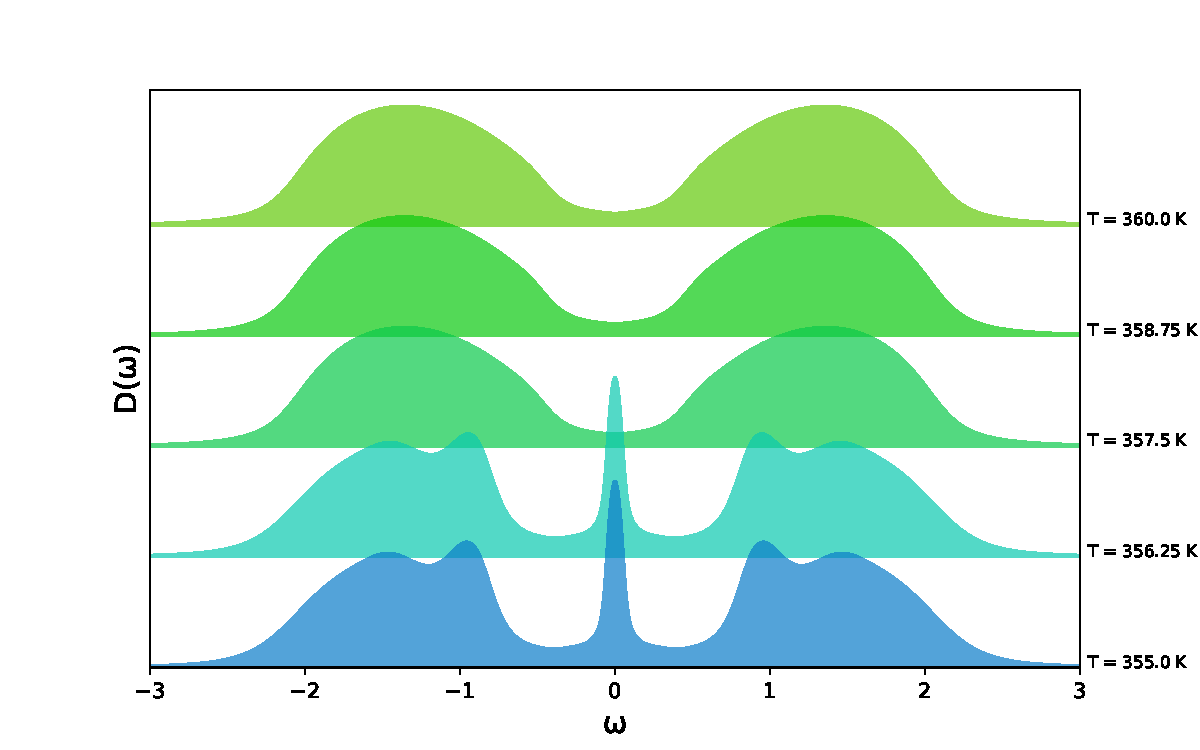
\includegraphics[width=1.00\textwidth]
		{pics/evolTDOS_IPT.pdf}
	\includegraphics[width=1.00\textwidth]
		{pics/evolTΣ2_IPT.pdf}
		\caption{(Atas) Evolusi DOS terhadap temperatur $T$, dan (Bawah) Evolusi dari nilai imajiner \textit{self-energy} dari variasi $T$ yang sama pada $U = 2.4$ dengan menggunakan metode penyelesaian impuritas teori iterasi pertubasi (IPT)}
\end{figure}	

Fase diagram paramagnetik yang dihitung dengan iterasi pertubasi teori ditunjukkan oleh gambar 4.3. Hasil yang diperoleh telah sesuai dengan literatur yang dihitung dengan metode penyelesaian yang lebih eksak seperti quantum monte-carlo\cite{ctqmc}. Hal ini dikarenakan IPT atau koreksi diagram hingga orde sudah cukup mampu untuk menyelesaikan kasus sistem material pada dimensi cenderung tinggi, dan pada kasus \textit{half-filling} dengan menampakkan perilaku transisi logam-isolator. Kita perhatikan bahwa, terdapat daerah ko-eksistensi logam-isolator dibawah parameter kritis $U_c,T_c$.  Koeksistensi mengisyaratkan masih terdapat adanya puncak eksitasi quasipartikel pada $\omega = 0$ dalam parameter tersebut, namun tidak sepenuhnya logam yang baik, dikarenakan jumlah keadaan quasipartikel sangat terbatas pada rentang energi tertentu saja.
\begin{figure}
	\centering
	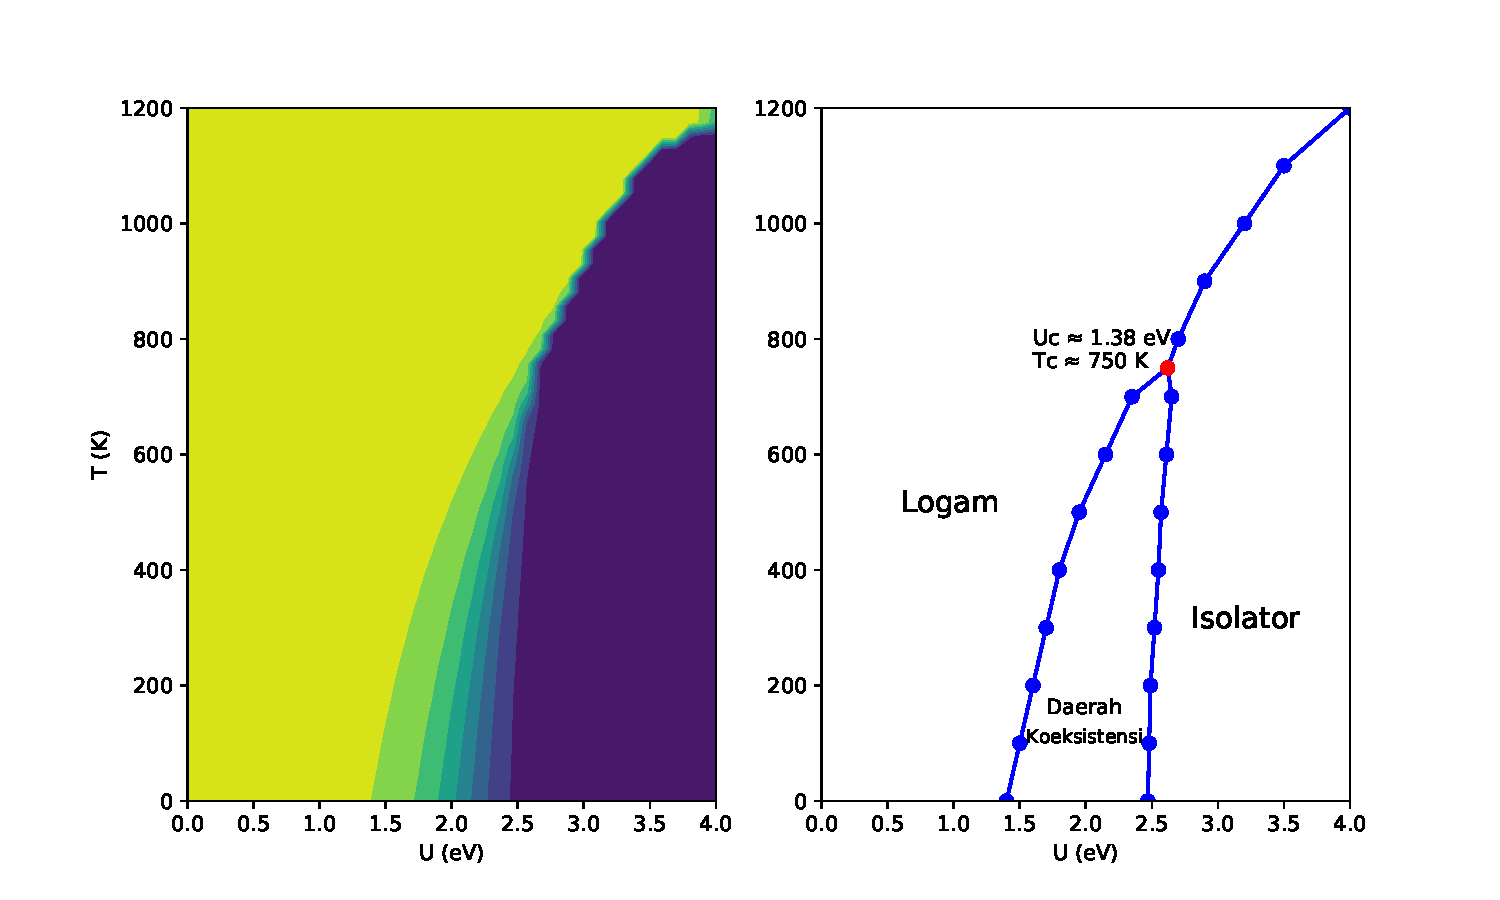
\includegraphics[width=1.00\textwidth]
		{pics/ipt_ph_diagram_param.pdf}
		\caption{Fase diagram paramagnetik transisi logam isolator yang dihitung dengan iterasi pertubasi teori (IPT)}
\end{figure}

Perhitungan pada kasus paramagnetik juga dilakukan untuk metode penyelesaian impuritas fluktuasi okupansi. Hal ini dilakukan untuk melihat perilaku \textit{self-energy} yang dihasilkan oleh fluktuasi okupansi. Evolusi DOS dan imajiner \textit{self-energy} diperlihatkan oleh gambar 4.4. Dengan memaksa sistem untuk berperilaku paramagnetik, melainkan okupnasi untuk kedua basis $\left\lbrace\uparrow,\downarrow\right\rbrace$ dipaksa sama, maka fluktuasi okupansi yang diberikan pada dasarnya tidak berpengaruh apa-apa. Hal ini dapat dikatakan karena jika kita mengidentifikasi fluktuasi dari probabilitas okupansi yang dihitung pada persamaan (3.32), yang diperlihatkan oleh gambar 4.5, terjadi simetrisasi antara nilai maksimum dan minimum, begitu juga untuk okupansi pada kedua basis $\left\lbrace\uparrow,\downarrow\right\rbrace$. Dengan menggunakan probabilitas okupansi yang simetri untuk kedua basis, sebagai perata-rataan fungsi Green yang dihitung pada persamaan (3.34), maka tidak heran jika fluktuasi okupansi ini pada dasarnya memberikan nilai rata-rata nol, atau mendekati nol. Pada kasus paramagnetik, hal ini memberikan kasus yang tak jauh berbeda dengan pendekatan medan rata-rata biasa.
\begin{figure}
	\centering
	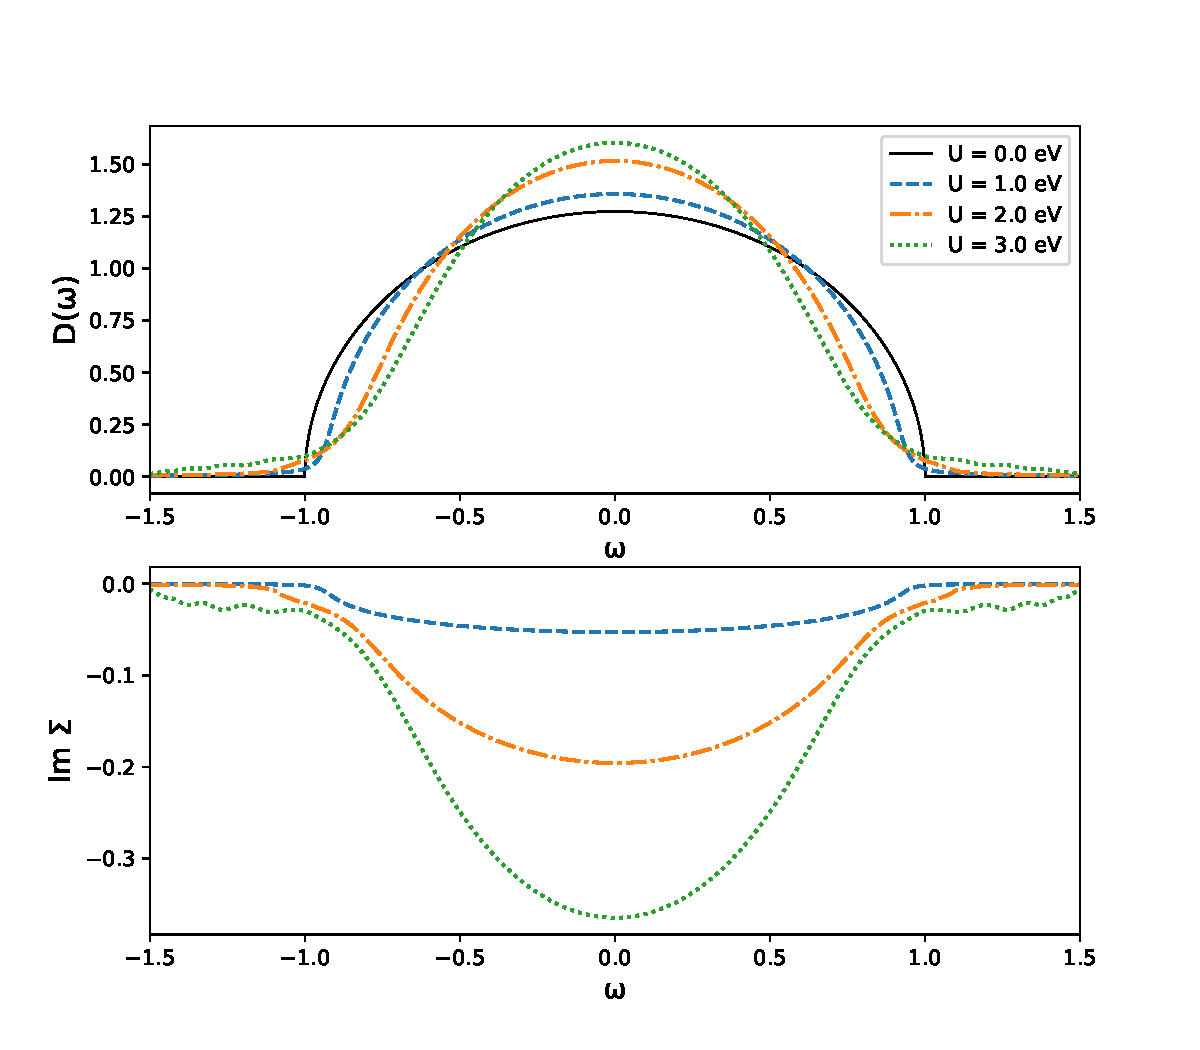
\includegraphics[width=1.00\textwidth]
		{pics/evolUDOS_OF.pdf}
		\caption{Evolusi DOS dan $\text{Im}\Sigma$ dari metode fluktuasi okupansi pada temperatur rendah $T = 50K$.}
	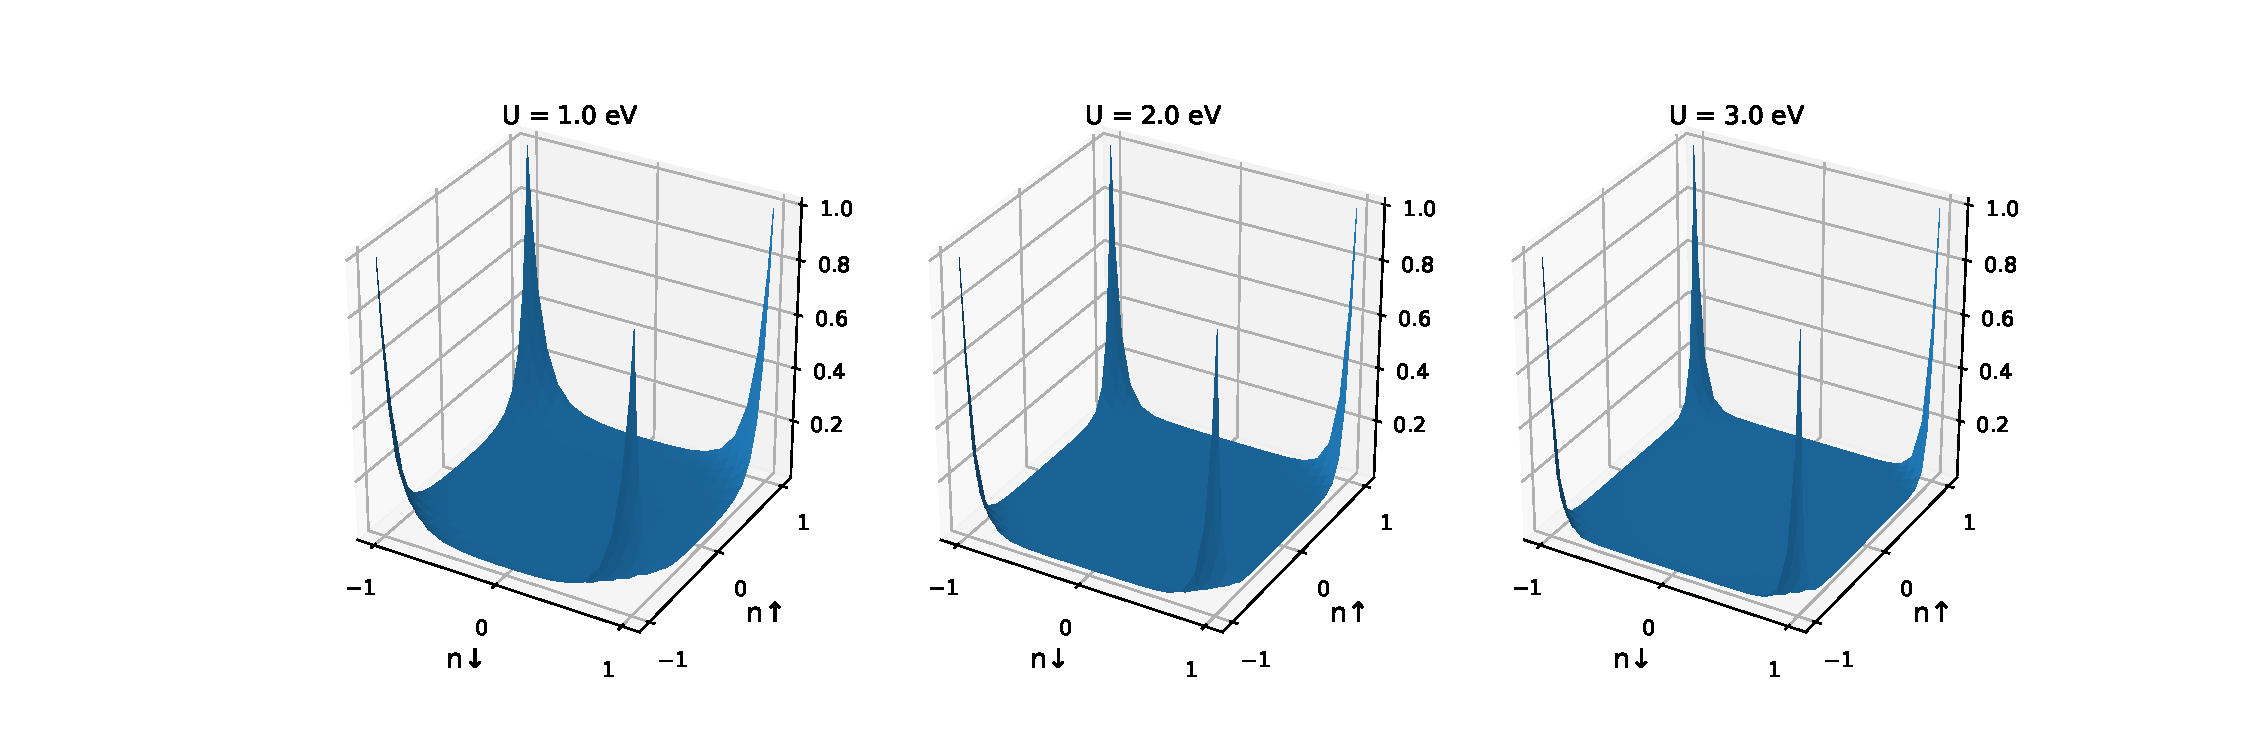
\includegraphics[width=1.00\textwidth]
		{pics/evolUProbabs_OF_PM.pdf}
		\caption{Probabilitas fluktuasi untuk kedua basis $\left\lbrace \uparrow, \downarrow \right\rbrace$ pada temperatur rendah $T = 50K$, dengan tiga variasi interaksi $U$.}
\end{figure}

Walaupun begitu, terlihat \textit{self-energy} tidak bernilai nol. Jika dilihat perilaku \textit{self-energy}, kurvanya menunjukkan seperti kurva semi-lingkaran seperti yang diperoleh dari kisi bethe. Hal ini bisa dipahami karena persamaan \textit{self-energy} didapat dari persamaan (3.35) sepenuhnya berasal dari informasi fungsi Green, baik impuritas maupun fungsi green kolam yang dua kuantitas itu sangat erat mengandung informasi kisi bethe. Hal ini juga diperkuat dengan hasil perata-rataan fungsi Green dari fluktuasi yang simetri sehingga kembali yang pada nilai yang tidak jauh berbeda dari nilai awal sebelum diberi fluktuasi. 
\begin{align}
G_{\text{ave}}(i\omega_n) \approx G_0(i\omega_n)
\end{align}
Perilaku \textit{self-energy} ini masih belum dapat diterima sebagai hasil fisis yang baik seperti halnya IPT yang didapat dari diagram orde-2. Okupansi fluktuasi sebagai metode penyelesaian impuritas pada kasus paramagnetik masih belum memberikan hasil yang memuaskan. 

%-----------------------------------------------------------------------------%
\section{Keadaan Antiferromagnetik}
%-----------------------------------------------------------------------------%
Terdapat keadaan dasar lain pada \textit{half-filling} yakni antiferomagnetik. Pada kalkulasi antiferomagnetik, orde satu diagram \textit{self-energy} atau perhitungan okupansi diperhitungkan. Perhitungan okupansi ini dilakukan di semua metode penyelesaian impuritas. Gambar 4.6 memperlihatkan total DOS dan DOS dari masing-masing basis $\text{Im} \Sigma$, untuk metode penyelesaian medan rata-rata. 

Gambar 4.6 memperlihatkan bahwa kedua spin memiliki jumlah keadaan energi yang saling berlawanan, hal ini akibat perbedaan nilai spin yang saling berlawanan. Dari sini terlihat pula, setiap spin memiliki DOS yang menyerupai DOS untuk kisi FCC. Hal tersebut dapat dijelaskan dengan bahwa setiap keadaan spin menempati satu sub-kisi (A) dan spin lain menempati sub kisi lain (B). Sehingga, pada kisi kubik, sub-sub kisi ini saling membentuk kisi FCC antara sub-kisi sejenisnya, sehingga tentu setiap spin memiliki bentuk DOS yang serupa. Namun terdapat bagian dari DOS dari masing-masing spin menempatin daerah energi berlawanan, hal ini dapat dijelaskan jika kita masih melihat elektron sebagai densitas fungsi gelombang, pada $U$ yang relatif rendah, densitas elektron masih berada sub kisi A dan sub kisi B, dengan densitas yang berbeda. Perilaku \textit{self-energy} sepenuhnya tidak bergantung dengan energi $\omega$, dimana bernilai konstan, dan memiliki nilai yang berlawanan antara \textit{self-energy} untuk basis $\left\lbrace\uparrow\right\rbrace$ dan basis $\left\lbrace\downarrow\right\rbrace$.
\begin{figure}
	\centering
	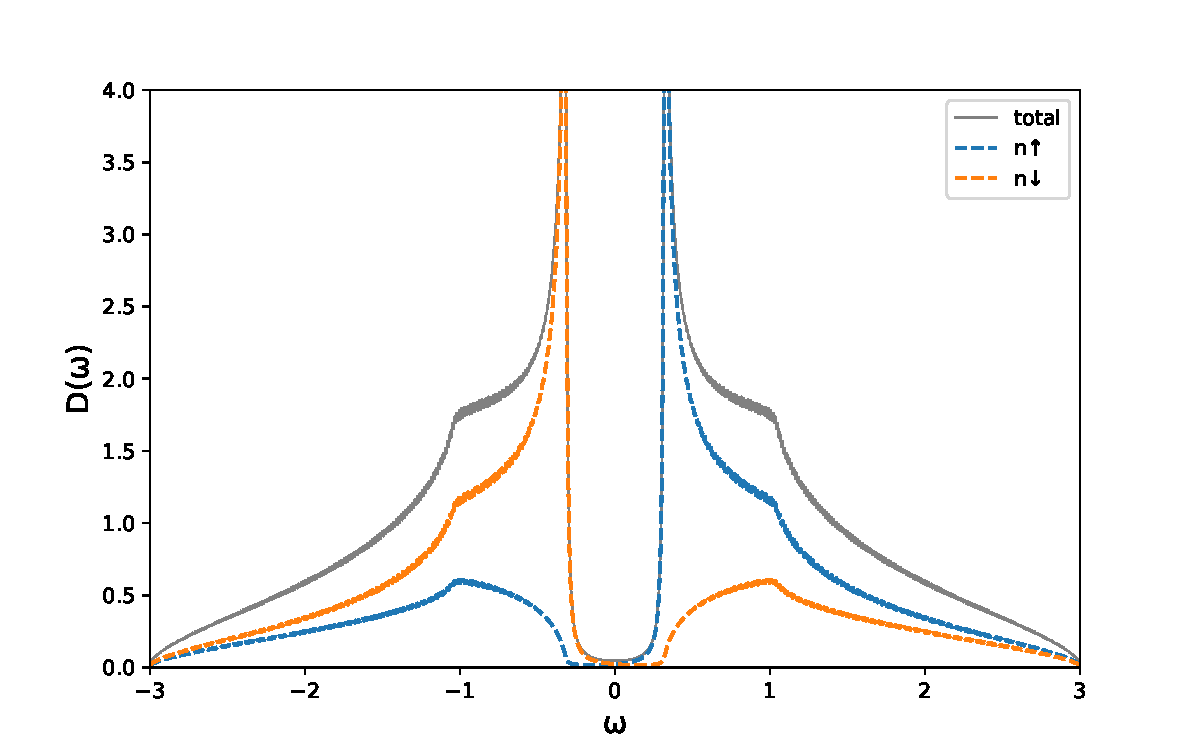
\includegraphics[height=0.5\textwidth, width=1.0\textwidth]
		{pics/dosupdown_MF_AF.pdf}
		\caption{Evolusi DOS terhadap $U$ pada temperatur $T = 0 K$ dan evolusi DOS terhadap $T$ pada $U = 1.5 eV$}
\end{figure}

Berikut juga diperlihatkan Gambar 4.7 evolusi DOS terhadap $U$ dan Temperatur $T$ dari perhitungan medan rata-rata. Formasi Gap sepenuhnya berasal dari perbedaan okupansi, dan pengaruh temperatur mengakibat besarnya eksitasi termal.
\begin{figure}
	\centering
	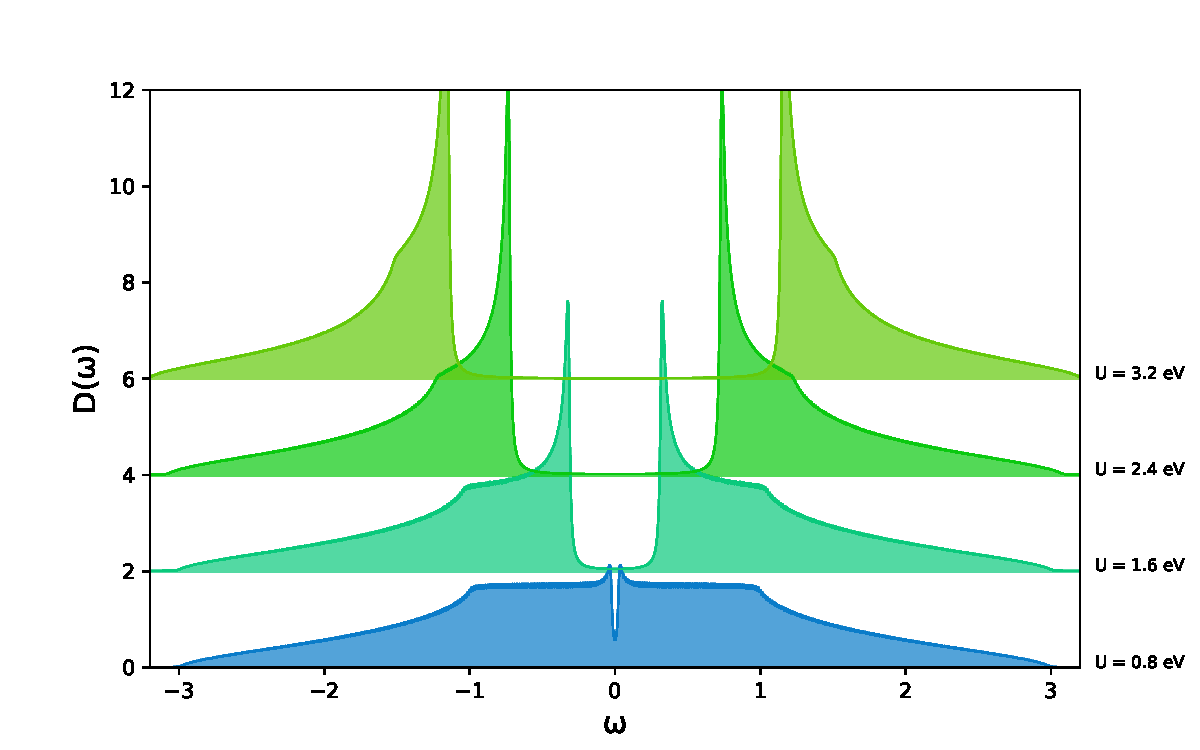
\includegraphics[height=0.4\textwidth, width=1.0\textwidth]
		{pics/evolUDOS_MF_AF.pdf}
	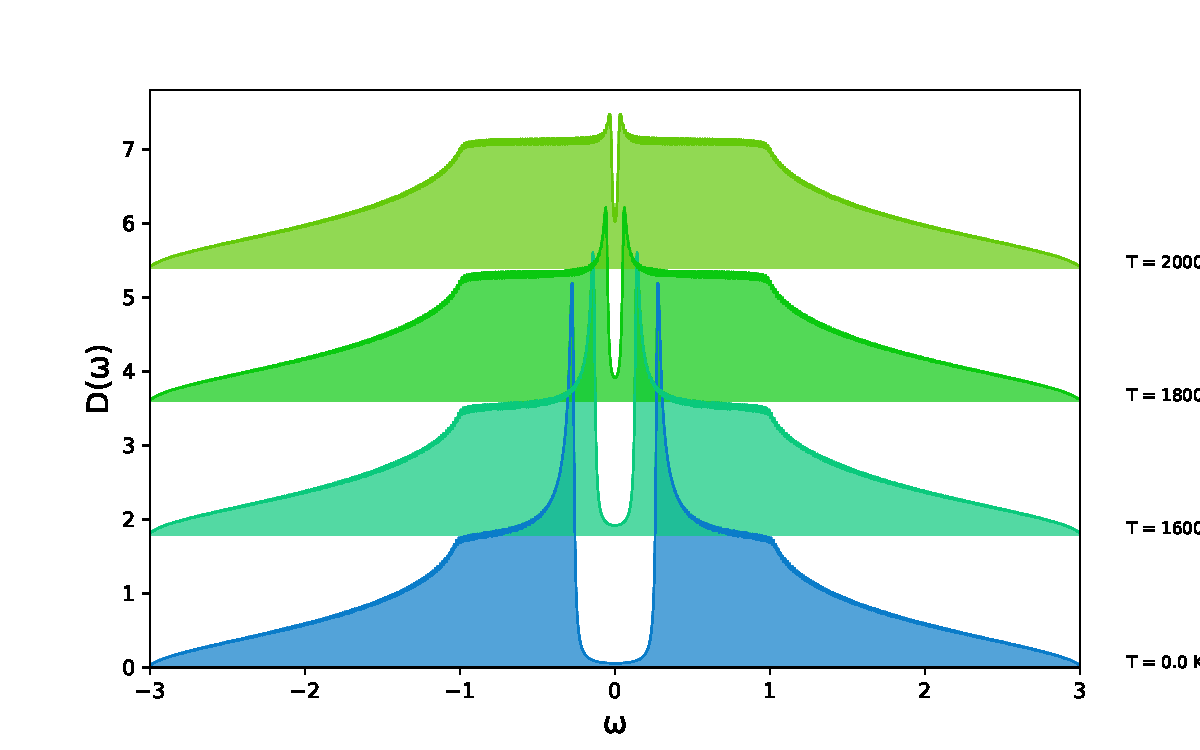
\includegraphics[height=0.4\textwidth, width=1.0\textwidth]
		{pics/evolTDOS_MF_AF.pdf}
		\caption{DOS dan DOS dari masing-masing basis orbital dengan perhitungan medan rata-rata, pada $U = 1.6 eV$ dan $T = 0.0 K$}
\end{figure}

Gambar 4.8 memperlihatkan perhitungan DOS melalui metode penyelesaian impuritas $IPT$ dengan $U = 2.0$ dan temperatur $T = 150 K$, DOS dua basis juga memiliki perilaku yang sama, namun sudah tidak sepenuhnya membentuk DOS FCC. Hal ini dikarenakan terdapat kontribusi diagram orde 2 pada \textit{self-energy}-nya. Pita DOS basis pada daerah energi berlawanannya (rentang energi negatif untuk basis $\uparrow$ dan positif untuk basis $\downarrow$) cenderung untuk menyebar. Hal ini bisa jika lihat pada $\text{Im}\Sigma$ yang memiliki dua puncak pada daerah energi relatif cukup tinggi, namun amplitudonya relatif kecil, yang mengindikasikan masih adanya kecendrungan untuk menyebar pada daerah energi tinggi, dan gap dari pita terbentuk berasal dari kontribusi diagram orde satu, atau nilai okupansi kedua basis dilihat perbedaan amplitudo dari $\text{Re}\Sigma$.
\begin{figure}
	\centering
	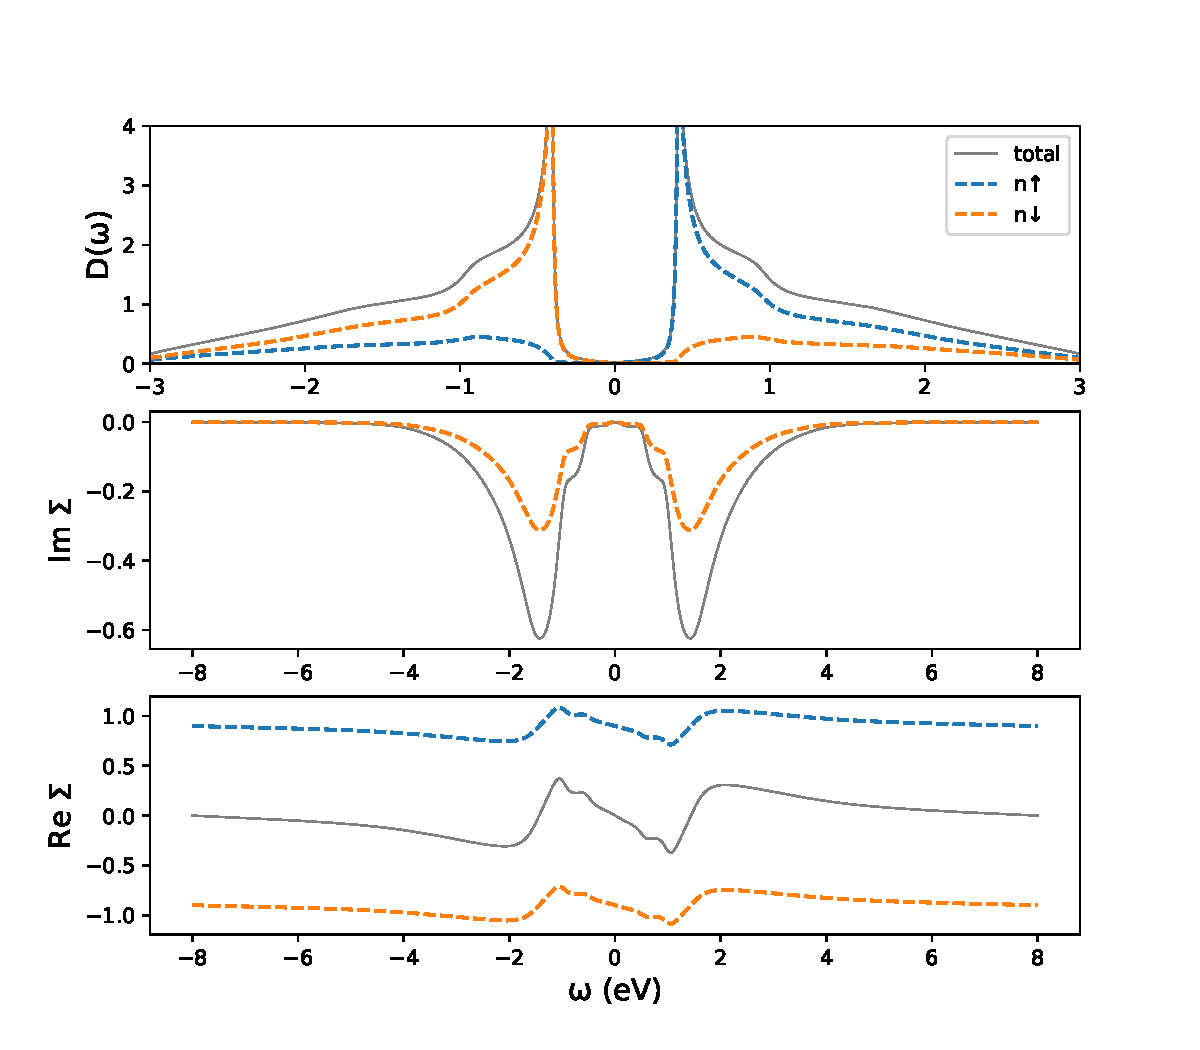
\includegraphics[width=1.0\textwidth]
		{pics/dosupdown_IPT_AF.pdf}
		\caption{DOS dan DOS dari masing-masing basis orbital dengan perhitungan IPT, pada $U = 2.0 eV$ dan $T = 150 K$}
\end{figure}

Selanjutnya, masih dalam IPT, kita lihat evolusi DOS untuk variasi interaksi lokal $U$. Evolusi DOS beserta $\textit{Im}\Sigma$ tersebut diperlihatknan pada gambar 4.9.
\begin{figure}
	\centering
	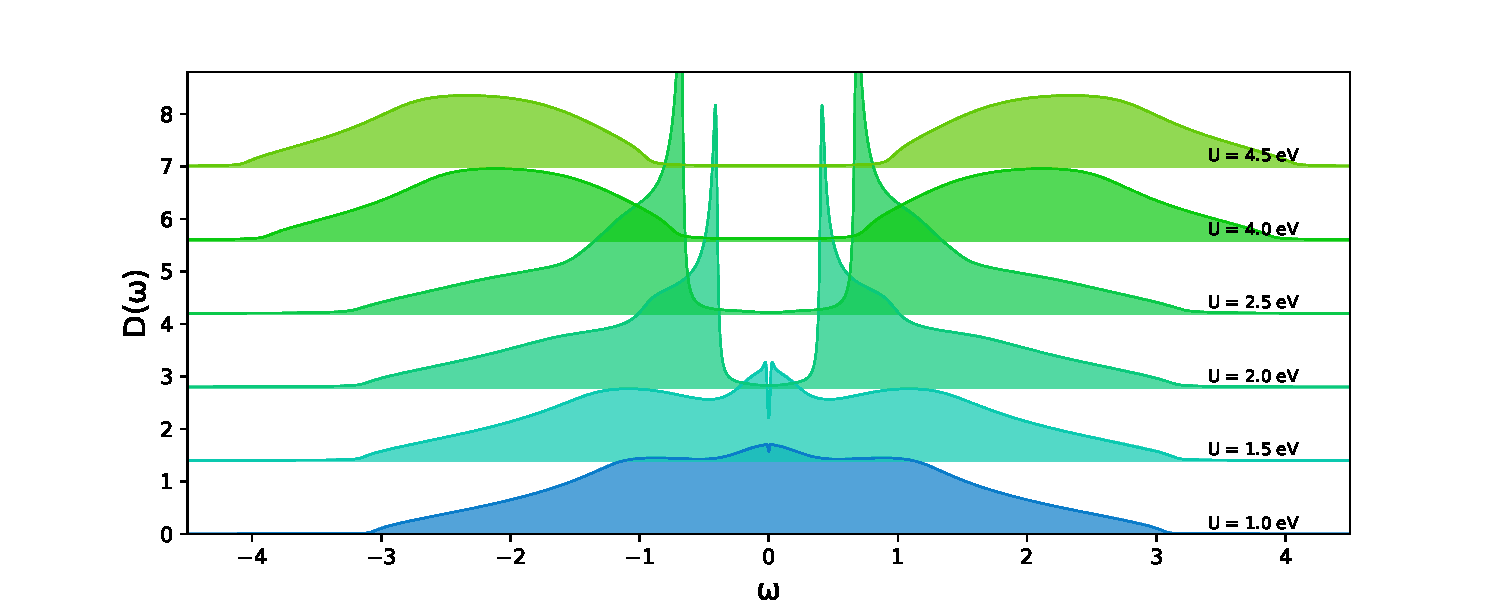
\includegraphics[width=1.0\textwidth]
		{pics/evolUDOS_IPT_AF.pdf}
	\includegraphics[width=1.0\textwidth]
		{pics/evolUΣ2_IPT_AF.pdf}
		\caption{Evolusi DOS dan nilai $\text{Im}\Sigma$ nya terhadap variasi $U$ pada temperatur $T = 150K$ menggunakan metode penyelesaian impuritas IPT}
\end{figure}

Pada $U$ yang relatif rendah, terdapat formasi quasipartikel, dan dalam hal ini okupansi untuk kedua basis masih relatif sama. Nilai $\text{Im}\Sigma$ menunjukkan alasan mengapa terjadi formasi quasipartikel sama halnya dengan kasus paramagnetik. Pada $U$ selanjutnya, formasi gap terjadi, dan ini berasal dari perbedaan nilai okupansi spin antara kedua kisi, dan puncak quasipartikel tidak lagi dapat dilihat akibat pengaruh formasi gap ini, namun dari nilai $\text{Im}\Sigma$ masih mengindikasikan seharusnya terdapat pita quasipartikel pada daerah energi fermi. Sedangkan pada $U$ yang tinggi, formasi gap tidak berasal dari perbedaan okupansi, melainkan kontribusi dari \textit{self-energy}, dimana dapat kita lihat nilai $\text{Im}\Sigma$ memiliki amplitudo yang sangat tinggi pada daerah energi fermi, yang kembali mengindikasikan tingginya energi interaksi pada energi rendah sehingga mengakibatkan lokalisasi.

Jika kita selanjutnya kita melihat evolusi DOS dengan variasi temperatur $T$, yang diperlihatkan oleh gambar 4.10. Formasi gap hilang dikarenakan berasal dari fluktuasi termal yang tinggi. Sedangkan jika dilihat dari kontribusi \textit{self-energy} orde dua, perubahan terjadi secara kontinu, dan memberikan formasi quasipartikel disaat hilangnya gap. Terjadi kompetisi quasipartikel dan perbedaan okupansi, pada temperatur transisi, ini mengakibatkan transisi secara mendadak pada keberadaan gap.
\begin{figure}
	\centering
	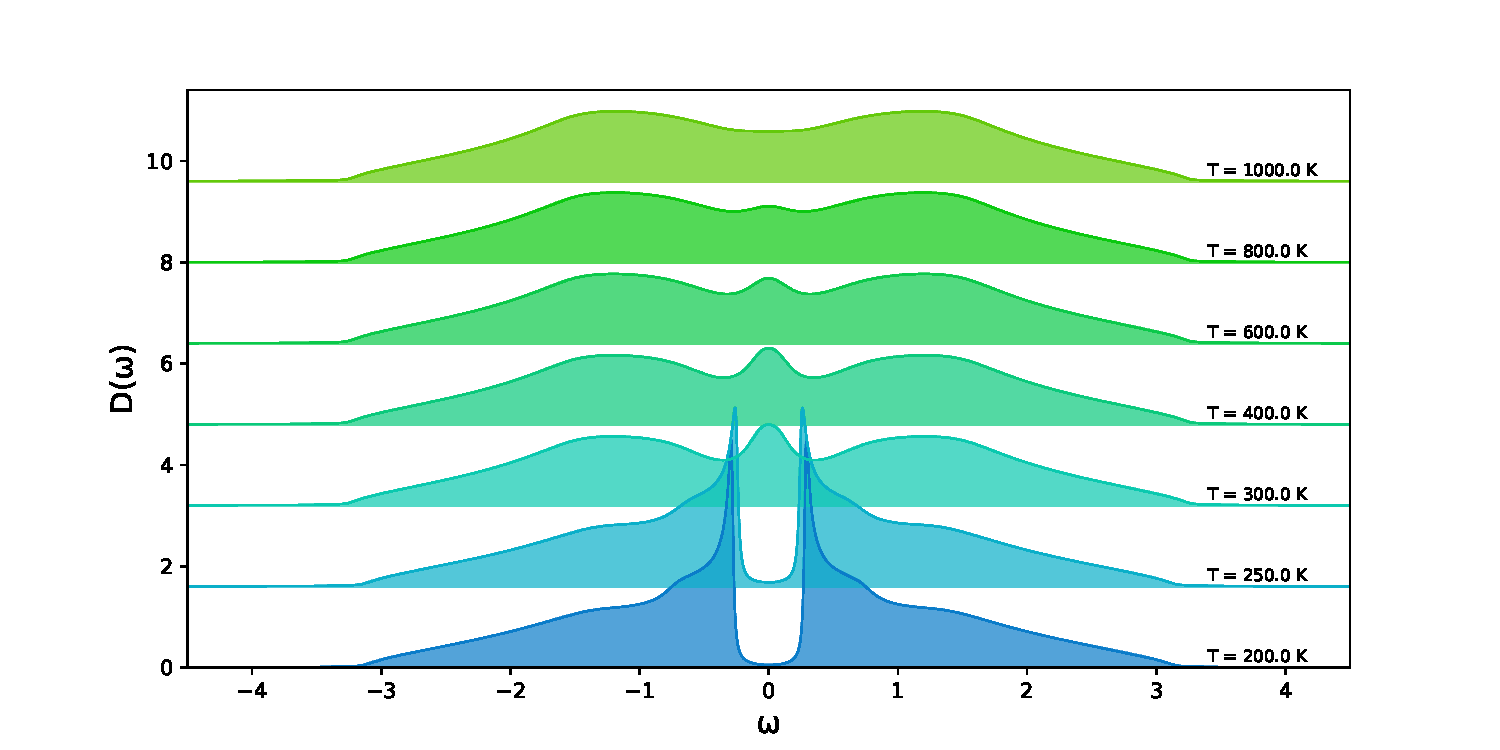
\includegraphics[width=1.0\textwidth]
		{pics/evolTDOS_IPT_AF.pdf}
	\includegraphics[height=0.4\textwidth, width=1.0\textwidth]
		{pics/evolTΣ2_IPT_AF.pdf}
		\caption{Evolusi DOS dan nilai $\text{Im}\Sigma$ nya terhadap variasi $T$ pada temperatur $U = 1.8$ eV menggunakan metode penyelesaian impuritas IPT}
\end{figure}

Pada perhitungan menggunakan okupansi fluktuasi murni, jika kita melihat DOS dan DOS masing-masing dari basis yang diperlihatkan gambar 4.11. Terlihat pada gambar tersebut dua puncak kecil pada daerah gap. Hal ini dapat kita lihat penyebabnya berasal dari $\Sigma$ yang semata-mata tidak hanya berasal dari kontribusi perbedaan okupansi, tetapi juga fluktuasinya. Tidak seperti halnya IPT yang seragam untuk kedua basis, nilai $\text{Im}\Sigma$ masing-masing memberikan nilai yang berbeda untuk kedua basis, hal ini wajar dikarenakan fluktuasi kedua basis memberikan nilai yang saling berlawanan. Fitur ini tentu tidak dimiliki oleh medan rata-rata biasa yang sama sekali menghilangkan fluktuasi okupansi didalamnya.

Evolusi DOS terhadap $U$ yang ditunjukkan oleh gambar 4.12 memperlihatkan pada $U$ yang rendah, terjadi paramagnetisme, yang kembali nilai $\text{Im}\Sigma$ merupakan bentuk yang sama dengan DOS dari kubik, sehingga pada $U$ yang rendah, belum dapat diterima secara fisis. Namun pada $U$ yang tinggi, dimana terjadi perbedaan okupansi yang berarti, nilai $\text{Im}\Sigma$ memberikan puncak-puncak tajam yang mengindikasi adanya fluktuasi interaksi elektron-elektron didalamnya.
\begin{figure}
	\centering
	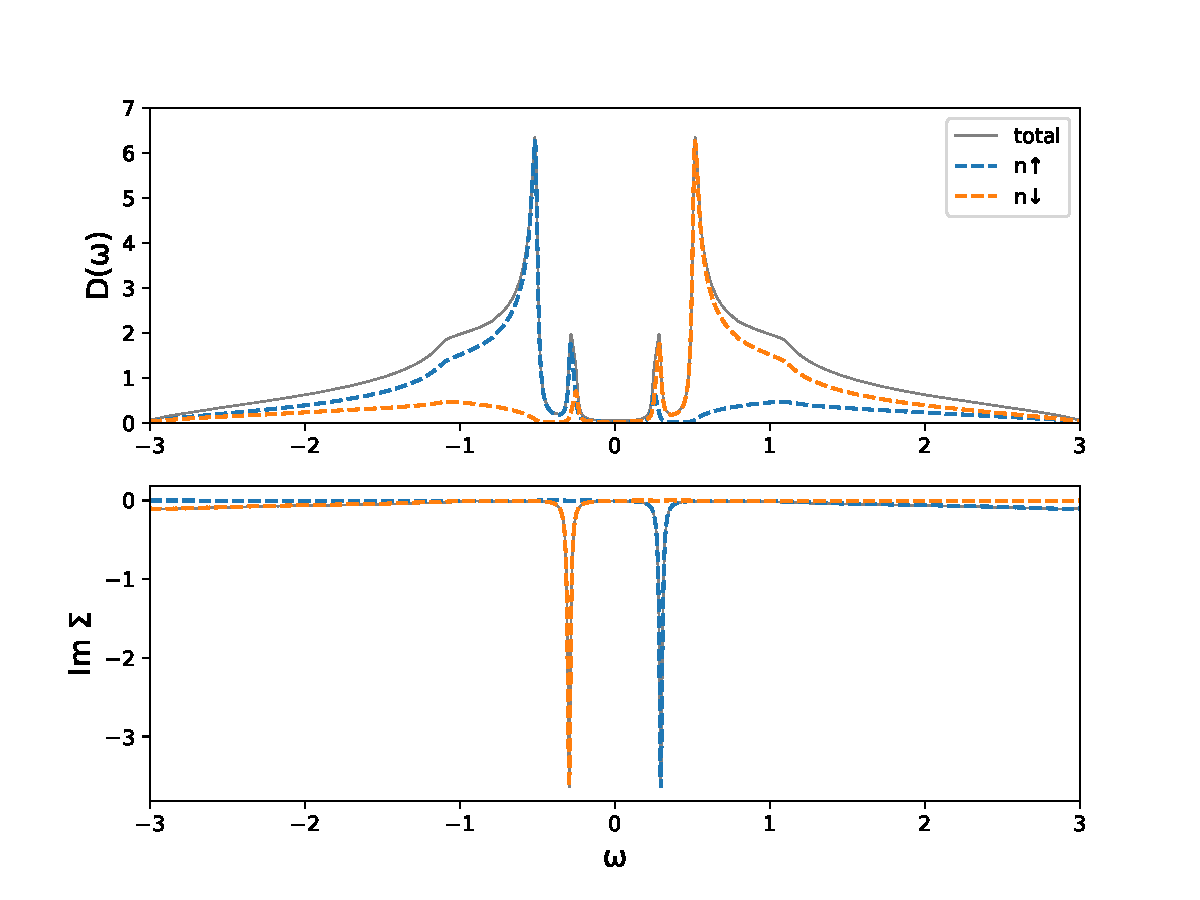
\includegraphics[width=0.9\textwidth]
		{pics/dosupdown_OF_AF.pdf}
		\caption{DOS dan DOS dari masing-masing basis orbital dengan perhitungan fluktuasi okupansi, pada $U = 2.0 eV$ dan $T = 20 K$}
\end{figure}

\begin{figure}
	\centering
	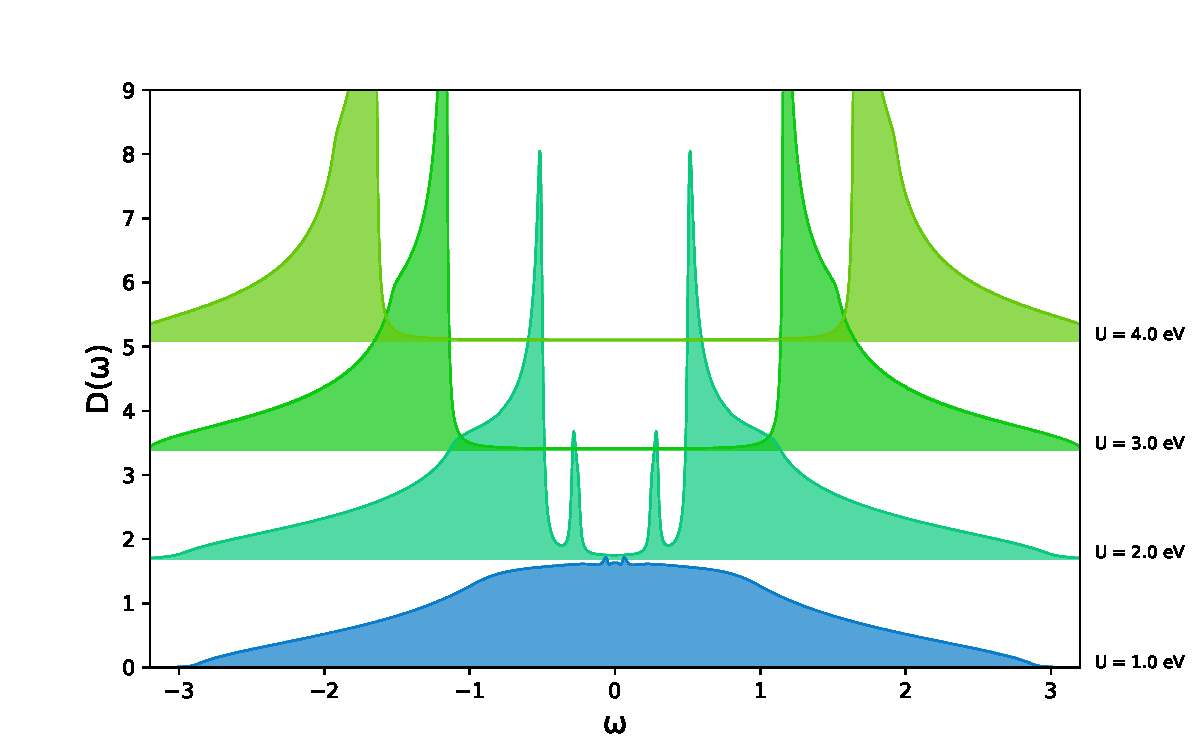
\includegraphics[height=0.4\textwidth, width=1.0\textwidth]
		{pics/evolUDOS_OF_AF.pdf}
	\includegraphics[height=0.35\textwidth, width=1.0\textwidth]
		{pics/evolUΣ_OF_AF.pdf}
		\caption{Evolusi DOS dan nilai $\text{Im}\Sigma$ nya terhadap variasi $T$ pada temperatur $U = 1.8$ eV menggunakan metode penyelesaian impuritas IPT}
\end{figure}

Selanjutnya evolusi DOS dan $\text{Im}\Sigma$ terhadap temperatur ditunjukkan oleh gambar 4.13. Hilangnya formasi gap dikarenakan fluktuasi termal, dan juga tingginya fluktuasi okupansi. Dapat kita lihat, kembali pada daerah paramagnetik, nilai $\text{Im}\Sigma$ membentuk nilai informasi yang sama dengan DOS paad kubik dengan nilai $U$ yang terbatas. Dapat dipastikan, segala keadaan paramagnetik pada okupansi fluktuasi, kurang memberikan hasil fisis yang tepat sebagai metode penyelesaian impuritas untuk DMFT.
\begin{figure}
	\centering
	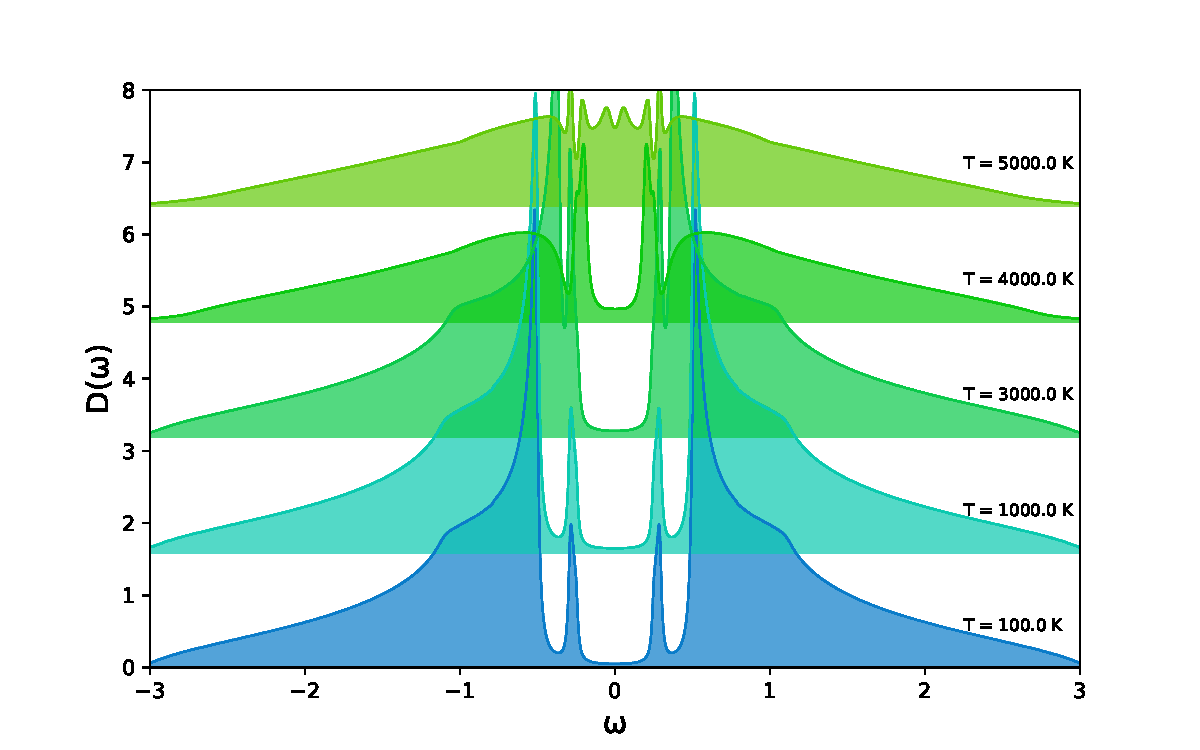
\includegraphics[height=0.4\textwidth, width=1.0\textwidth]
		{pics/evolTDOS_OF_AF.pdf}
	\includegraphics[height=0.35\textwidth, width=1.0\textwidth]
		{pics/evolTΣ_OF_AF.pdf}
		\caption{Evolusi DOS dan nilai $\text{Im}\Sigma$ nya terhadap variasi $T$ pada temperatur $U = 1.8$ eV menggunakan metode penyelesaian impuritas IPT}
\end{figure}

\subsection{Okupansi Fluktuasi sebagai Koreksi IPT}
Dari hasil keadaan paramagnetik tersebut, kami termotivasi untuk menjadi okupansi fluktuasi bukan sebagai metode penyelesaian impuritas DMFT yang utama, melainkan sebagai koreksi okupansi dari IPT, selanjutnya akan disebut sebagai IPT+OF. Perhitungan dilakukan sesuai diagram algoritma yang dijelaskan pada bab 3, dimana hasil dari IPT digunakan sebagai nilai masukan untuk okupansi fluktuasi. 

Gambar 4.14 memperlihatkan DOS total dan DOS untuk kedua basis, serta nilai $\text{Im}\Sigma$ pada $U$ yang relatif tinggi yakni $U = 4.0$ eV. Dapat kita lihat bahwa informasi DOS mengisyaratkan bahwa sistem belum menjadi paramagnetik, melainkan antiferomagnetik, tetapi bentuk kurvanya berbeda dari antiferomagnetik yang ditunjukkan oleh DOS yang hanya akibat perbedaan okupansi. Nilai $\text{Im}\Sigma$ juga memberikan perbedaan \textit{shift} untuk kedua basis yang berbeda, dimana tidak sepenuhnya bernilai sama seperti yang didapat dari IPT. Dari IPT kita lihat bahwa gap terbentuk akibat kompetisi perbedaan okupansi dan kuatnya interaksi pada energi rendah, namun pada IPT+OF gap dapat terjadi akibat koeksistensi dari perbedaan okupansi dan koreksi 
\textit{self-energy} diagram orde dua. Hilangnya karakter gap yang hanya dikarenakan perbedaan okupansi juga disebabkan oleh fluktuasi termal dimana pada gambar 4.14 nilai temperatur $T = 150K$.
\begin{figure}
	\centering
	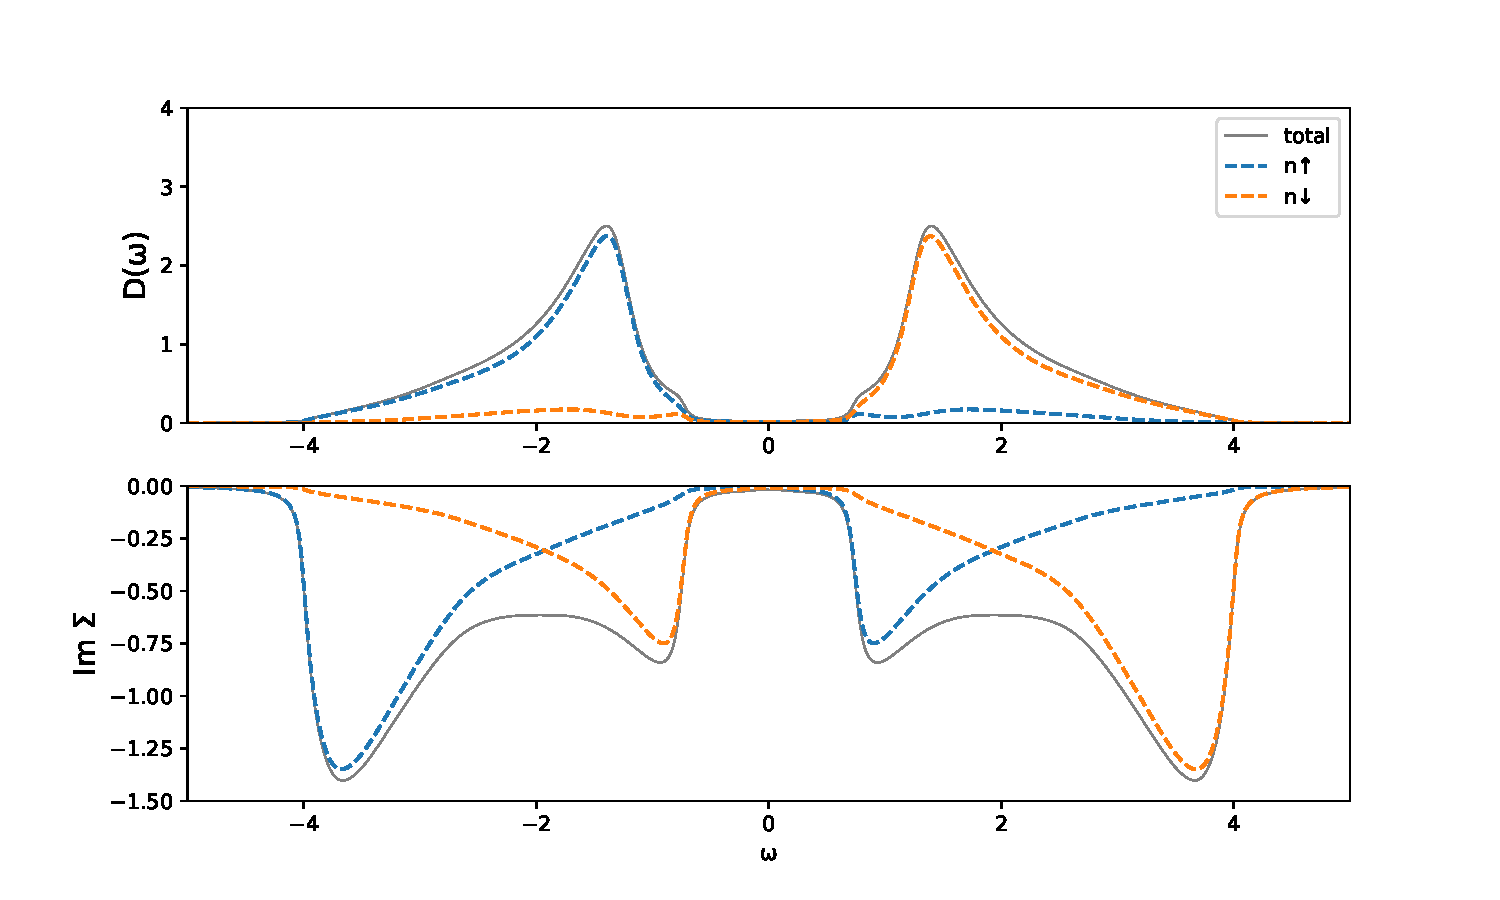
\includegraphics[width=1.0\textwidth]
		{pics/dosupdown_OFIPT_AF.pdf}
		\caption{DOS dan DOS dari masing-masing basis orbital dengan perhitungan IPT+OF, pada $U = 4.0 eV$ dan $T = 150K K$}
\end{figure}

Gambar 4.15 memperlihatkan evolusi DOS dan $\text{Im}\Sigma$ dari IPT+OF terhadap $U$, dimana pada $U$ yang relatif tinggi, sistem masih mempertahankan sifat antiferomagnetismenya walaupun kondisi fisis sudah berbeda dari antiferomagnetisme akibat perbedaan okupansi biasa. Jika dilihat perilaku $\text{Im}\Sigma$, pada $U$ relatif rendah, ini memiliki kontribusi seperti dari yang diberikan oleh OF, karena kontribusi IPT berada pada rentang amplitudo yang rendah untuk energi yang rendah. Sedangkan, pada $U$ yang tinggi, terjadi koeksistensi keduanya.
\begin{figure}
	\centering
	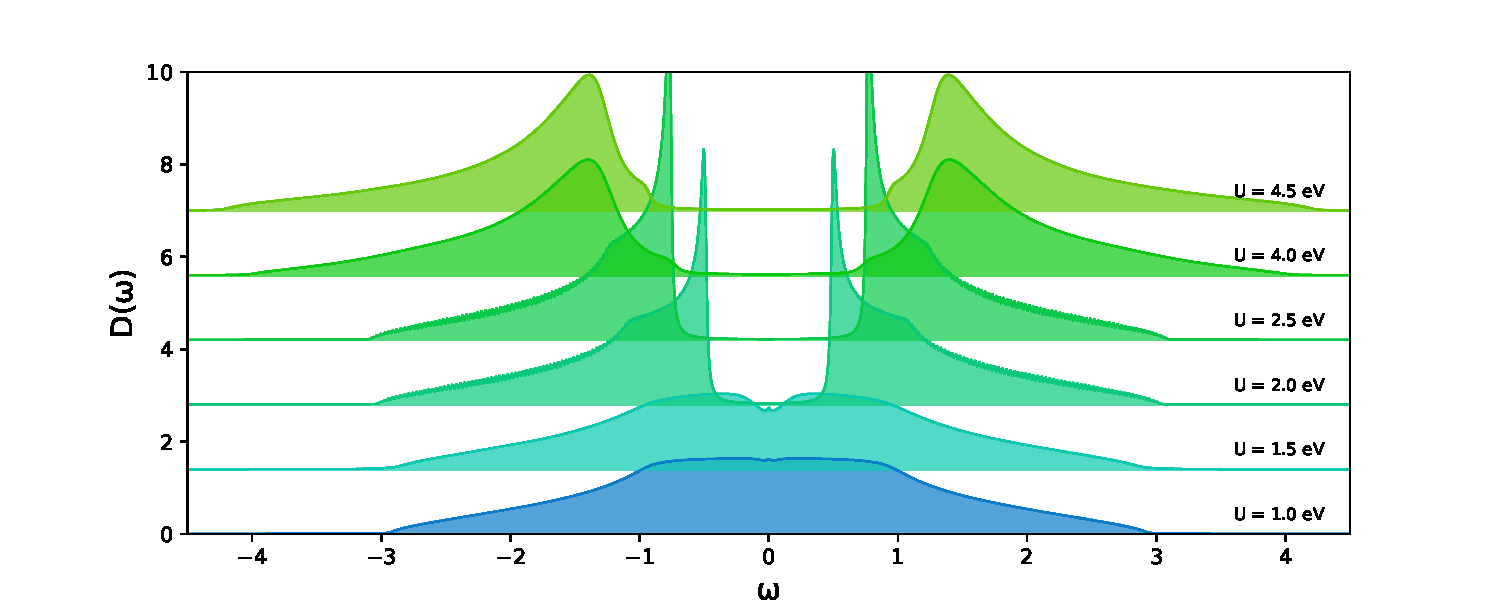
\includegraphics[height=0.4\textwidth, width=1.0\textwidth]
		{pics/evolUDOS_OFIPT_AF.pdf}
	\includegraphics[height=0.35\textwidth, width=1.0\textwidth]
		{pics/evolUΣ2_OFIPT_AF.pdf}
		\caption{Evolusi DOS dan nilai $\text{Im}\Sigma$ nya terhadap variasi $U$ pada temperatur $T = 150 K$ eV menggunakan metode penyelesaian impuritas IPT+OF}
\end{figure}

\begin{figure}
	\centering
	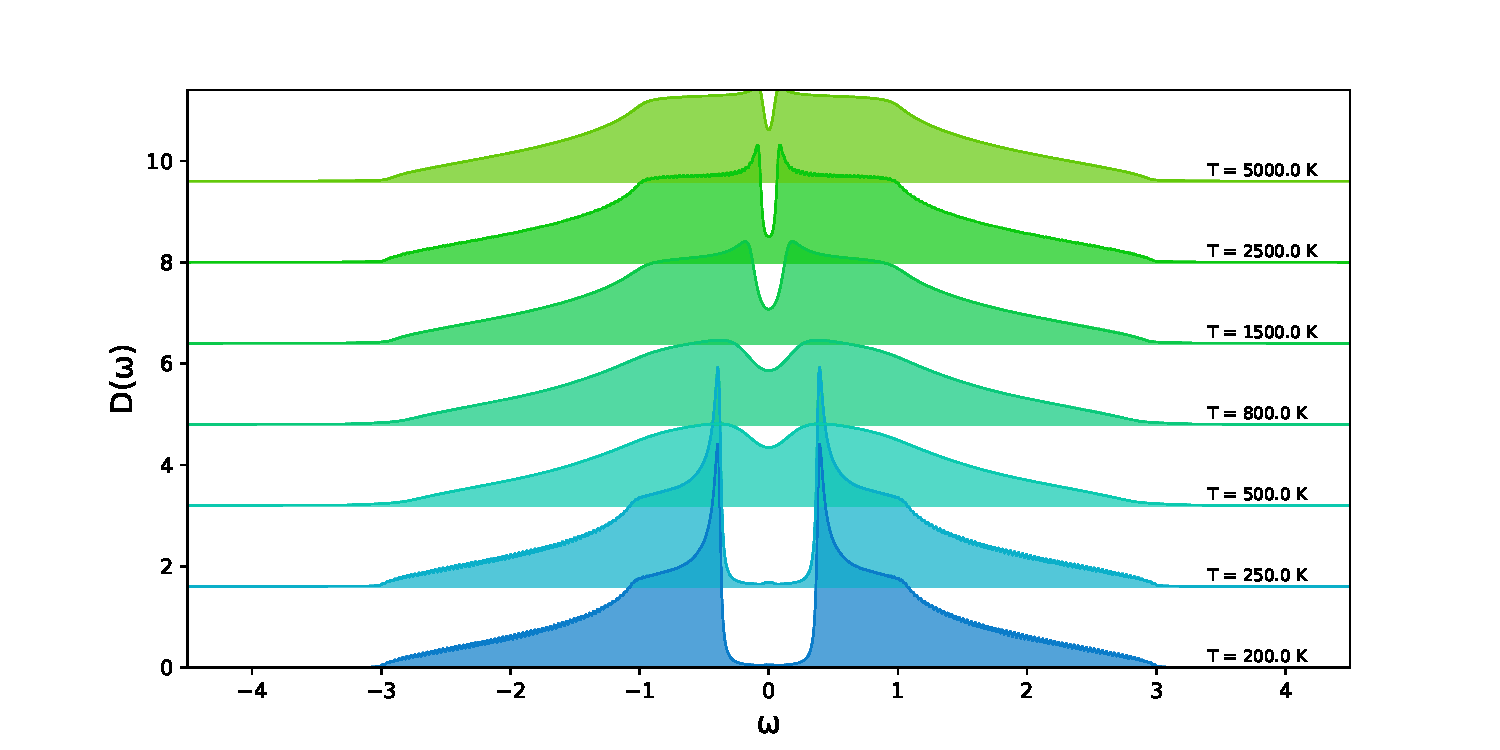
\includegraphics[height=0.4\textwidth, width=1.0\textwidth]
		{pics/evolTDOS_OFIPT_AF.pdf}
	\includegraphics[height=0.3\textwidth, width=1.0\textwidth]
		{pics/evolTΣ2_OFIPT_AF.pdf}
		\caption{Evolusi DOS dan nilai $\text{Im}\Sigma$ nya terhadap variasi $T$ pada temperatur $U = 1.8$ eV menggunakan metode penyelesaian impuritas IPT}
\end{figure}

Gambar 4.16, memperlihatkan evolusi DOS dan $\text{Im}\Sigma$ dari IPT+OF terhadap $T$. Kita lihat bahwa evolusi temperatur pada daerah $T = 200 K$ hingga transisi pada $T = 500K$ merupakan kontribusi dari IPT. Namun, menariknya, pada temperatur yang semakin tinggi, terbentuk pseudogap yang semakin besar, dan kembali tertutup seperti layaknya dari perhitungan medan rata-rata. Hal ini dapat dilihat dari $\text{Im}\Sigma$ yang dimana kontribusi dari OF memiliki peran besar untuk menampilkan perilaku gap DOS sebagai perbedaan okupansi.

Perhitungan IPT+OF memberikan hasil yang menarik, selain memberikan perilaku perbedaan okupansi untuk nilai $\text{Im}\Sigma$, tetapi juga memberikan daerah koeksistensi kontribusi dari gap yang terbentuk akibat perbedaan okupansi dan \textit{self-energy} pada orde kedua. Jika kita melihat perilaku evolusi magnetisme subkisi pada ketiga metode, medan rata-rata, IPT, dan IPT+OF, kita mendapatkan hasil yang menarik, hal ini diperlihatkan pada gambar 4.17. Perubahan pada perhitungan medan rata-rata terjadi secara kontinu, hal ini magnetisme berkolerasi linear terhadap terbentuknya gap, sehingga magnetisme dapat dihitung dengan persamaan gap untuk medan rata-rata\cite{staudt}. Sedangkan pada IPT, akibat koreksi orde 2 dan kompetisinya terhadap perbedaan okupansi, terjadi transisi secara mendadak, baik terhadap perubahan $U$ dan $T$. Selanjutnya pada IPT+OF, dimana fluktuasi okupansi digunakan sebagai koreksi IPT, pada $U$ dan $T$ yang relatif rendah, nilai IPT dan IPT+OF cukup \textit{fitting} satu sama lain, namun terjadinya transisi AF-PM, fluktuasi okupansi berperan menahan terjadinya transisi secara tajam. Akibat adanya fluktuasi okupansi, keadaan PM tidak semerta-merta dapat dicapai dengan mudah.

Hasil utama pekerjaan skripsi ini diperlihatkan dari gambar 4.18. Walaupun dari perilaku magnetisme IPT+OF yang diperlihatkan oleh gambar 4.17, sayangnya diagram fasa magnetisme pada IPT+OF tidak memberikan koreksi yang cukup berarti untuk IPT dalam mengoreksi fasa yang mendekati eksak, yakni $U$ kecil mengikuti persamaan gap dari pendekatan medan rata-rata, dan $U$ yang besar diambil dari batas heisenberg. Perhitungan menggunakan metode penyelesaian impuritas CTQMC\cite{ctqmc} juga diperlihatkan sebagai pembanding, dimana terlihat bahwa metode penyelesaian impuritas menggunakan ctqmc cukup mampu dalam memprediksi diagram fasa kisi kubik pada DMFT, data diambil dari referensi\cite{staudt}.
\begin{figure}
	\centering
	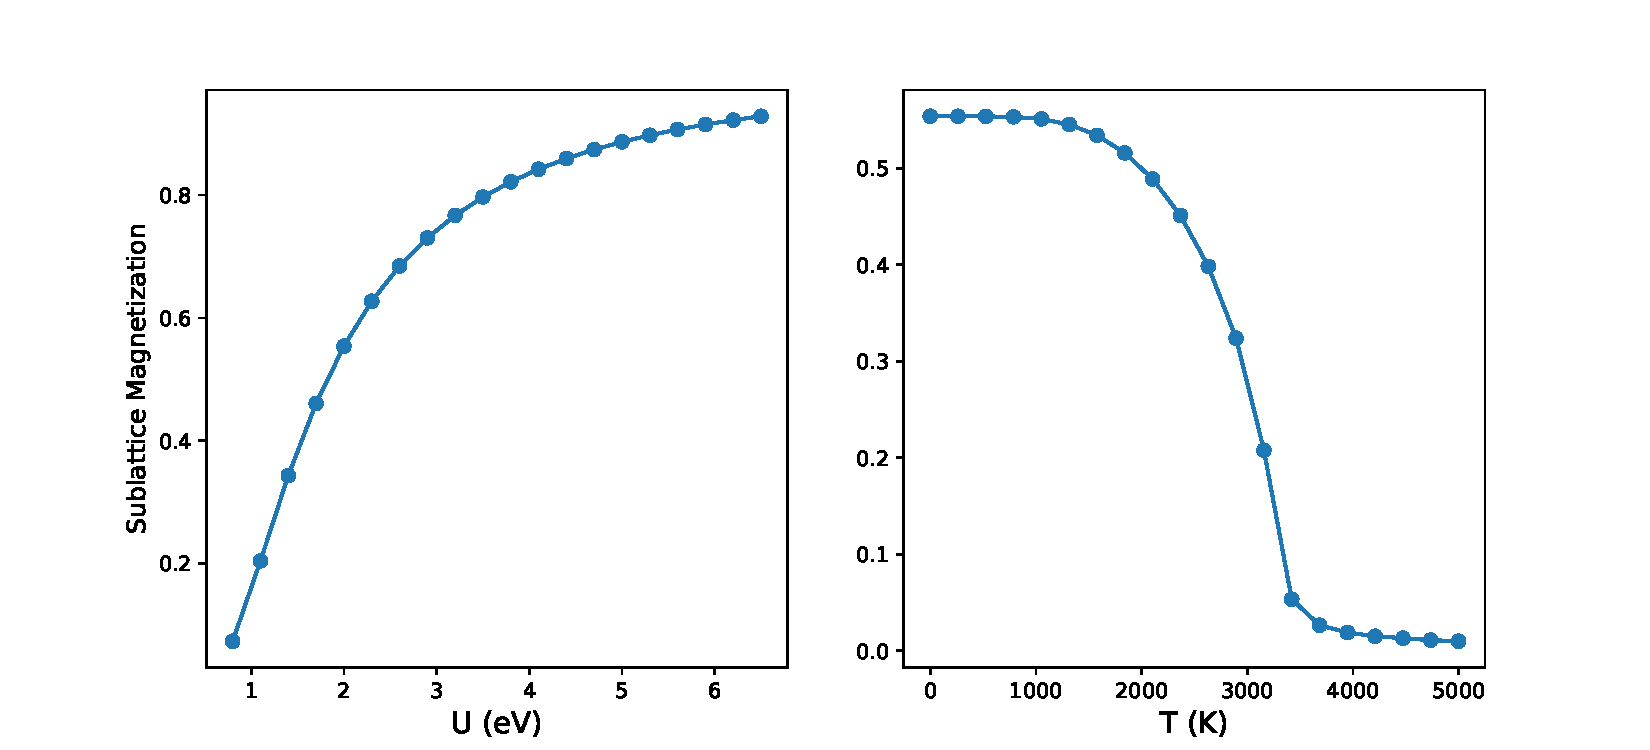
\includegraphics[height=0.5\textwidth, width=1.0\textwidth]
		{pics/magnetization_MF_AF.pdf}
	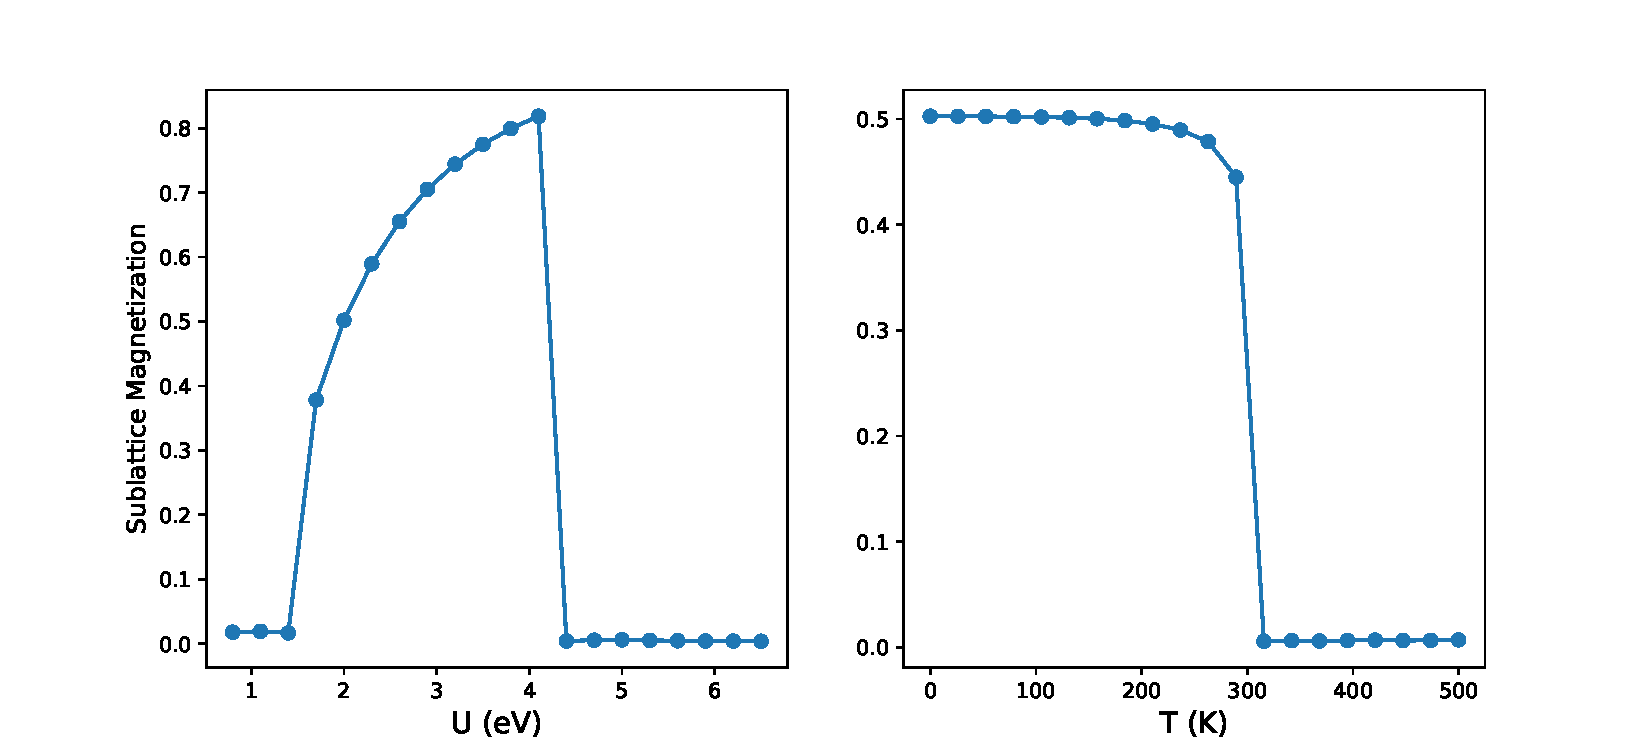
\includegraphics[height=0.5\textwidth, width=1.0\textwidth]
		{pics/magnetization_IPT_AF.pdf}
	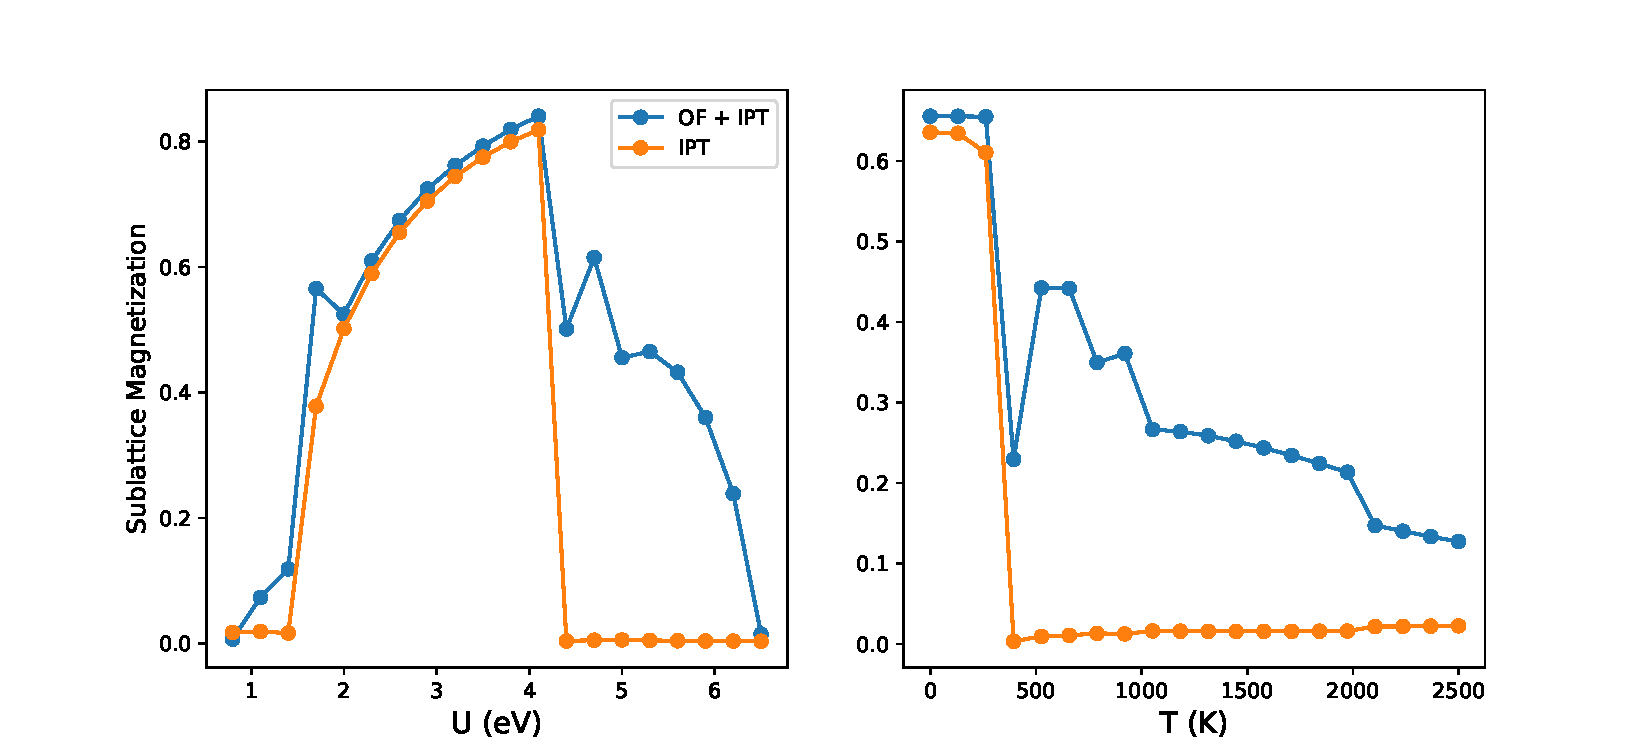
\includegraphics[height=0.5\textwidth, width=1.0\textwidth]
		{pics/magnetization_OFIPT_AF.pdf}
		\caption{(Atas) Evolusi magnetisme dari subkisi terhadap $U$ dan $T$ yang dilakukan dengan metode medan rata-rata. (Tengah) Evolusi magnetisme dari subkisi terhadap $U$ dan $T$ yang dilakukan dengan IPT. (Bawah) Evolusi magnetisme dari subkisi terhadap $U$ dan $T$ yang dilakukan dengan metode IPT+OF.}
\end{figure}
\begin{figure}
	\centering
	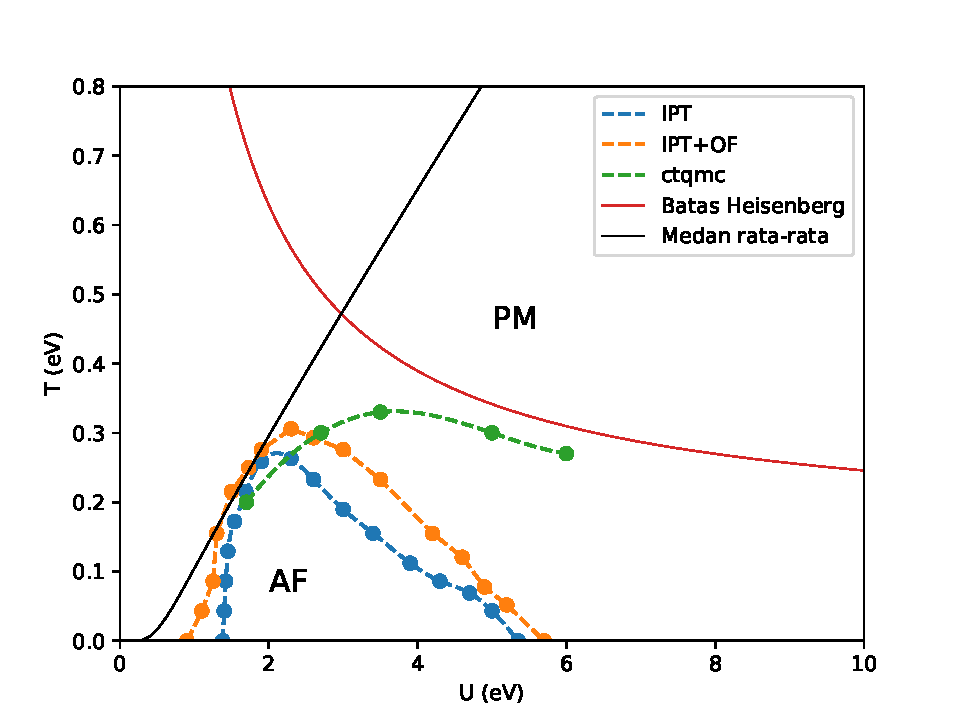
\includegraphics[width=1.0\textwidth]
		{pics/phasediagram_AF.pdf}
		\caption{Diagram Fasa Magnetisme untuk kisi 3D Kubik pada model Hubbard. Kalkulasi dari skripsi ini dilakukan untuk IPT dan IPT+OF. Data CTQMC diambil dari ref\cite{staudt}.}
\end{figure}